
\chapter{Concept and Design}
\label{cha:conceptanddesign}

\section{General}

\section{Requirements and Challenges}

\subsection{Requirements}

\subsubsection{GDPR compliance}
\label{subsubsec:GDPR_compliance}
The General Data Protection Regulation (GDPR) is a regulation by the European Parliament, Council of the European Union and the European Commission focused on strengthening EU citizens digital privacy.  Its main focus is on giving citizens control over their digital personal information and simplifying the regulatory environment for multinational corporations. However it also adds a strict data compliance regime, by penalizing transgressions with up to 4\% worldwide turnover\cite{gdpr}. Furthermore this regulation does not have to be verified by each EU's regulatory body, since it is a EU regulation, compared to an EU directive which has to be ratified by each EU signatory state.

\section{Challenges}
\label{sec:challenges}

\subsection{Security Goals}
\label{sec:securityGoals}

Designing a identity management systems comes with various legal implications. We are referring here to § 9 “Technical and organizational actions” in the “Federal Data Protection Act”\footnote{Translated from the German language “Bundesdatenschutzgesetz”} were an identity management system shell enforce all necessary measures to protect identity information.\cite{bdsg}

So we will focus on the following security goals:
\begin{enumerate}
\item \textbf{Confidentiality:} Data shell be secured on its transmission. This includes the blockchain and communication over the internet. 
\item \textbf{Integrity:} The integrity of the data needs to be assured so that no entity can change identity information without knowledge. 
\item \textbf{Authenticity:} Identity information are protected against unauthorized access. 
\item \textbf{Non-Repudiation:} No entity can deny having taken an action.
\item \textbf{Privacy:} The privacy of a user is preserved while interacting with the system. 
\end{enumerate}

We further also see the blockchain as a world open readable ledger were everyone can read transactions or information stored on the blockchain. So interactions with the blockchain need to ensure to not expose any identity information. 
It is not allowed to store hashes or encryption of claim in the blockchain, since it is a tamper-proof data storage, information can not be removed once written. So if the hash or encryption gets broken the identity information is leaked and can not be removed.  

\subsection{User Acceptance}
\label{sec:userAcceptance}

TODO Oskar
Switching from offline to online identity is an unspecified burden that falls into the eye of a common pleb.
Especially for elderly and uneducated the imagination of not having a piece of paper with an id and not having a central
institution that takes care of one's identity is suspect, if not horrifying.
Not only the lack of a trusted party but also the concept of blockchain, smart contracts and all of its gists are unknown
to most people. This leads to further distrust in the system.

By introducing such system, a lot of clarification for non-technical people and common folks therefore needs to have a
high priority.

Without understanding the process and system, users run the risk of being exploited and not being aware of what information
they are currently sharing.

\subsection{Economic feasibility}
\label{sec:economicFeasibility}
In order for a new system to become succesful, it is imperative that it is econimically feasible. Its total cost of ownership should be comparable to or even lower than the system it is replacing.
However the total cost of ownership of an identity system where the blockchain is used for storing transactional information is extremely difficult to gauge. This is in part because it is a "living platform" which is constantly being changed, but also because of the volatility of cryptocurrencies.\cite{elendner2016cross}
Due to cryptos nature it is difficult to keep costs stable or predictable, since accurate models are still actively being worked on.\cite{catania2018predicting} The slightest change in financial regulation, bad press, or just negative comments in social media can crash their prices.\cite{kim2016predicting}
In contrast their prices can also rise in an astonishing fashion because of aforementioned reasons. 
This projects aim however has not been to create an economically feasible platform, but a simple demonstrator, showcasing that blockchain technologies could be adapted to suit the societal needs of a digitalized society. \projectName{} can be used as a digital alternative to an already existing non-digital system.
However before a full deployment could take place further development is necessary to minimize all costs associated with the interactions with the blockchain.
As an alternative solution however it would be possible to replace the public blockchain with a governmentally run private network. This would reduce the costs of transactions by giving the owning entity full control over all costs associated with the blockchain transactions.
This however would also cancel the independent miners motivation to be part of the system. Creating the need for different remuneration concepts or even state owned miners. These proposals however would introduce new risks into the system by defining a single trust anchor for the entire system. 

\section{Processes}

\subsection{Registration}
In order to be part of our distributed digital identity system that we envisioned, it is necessary to register with it first. The registration process consists of the following steps:

\begin{figure}[ht]
\centering
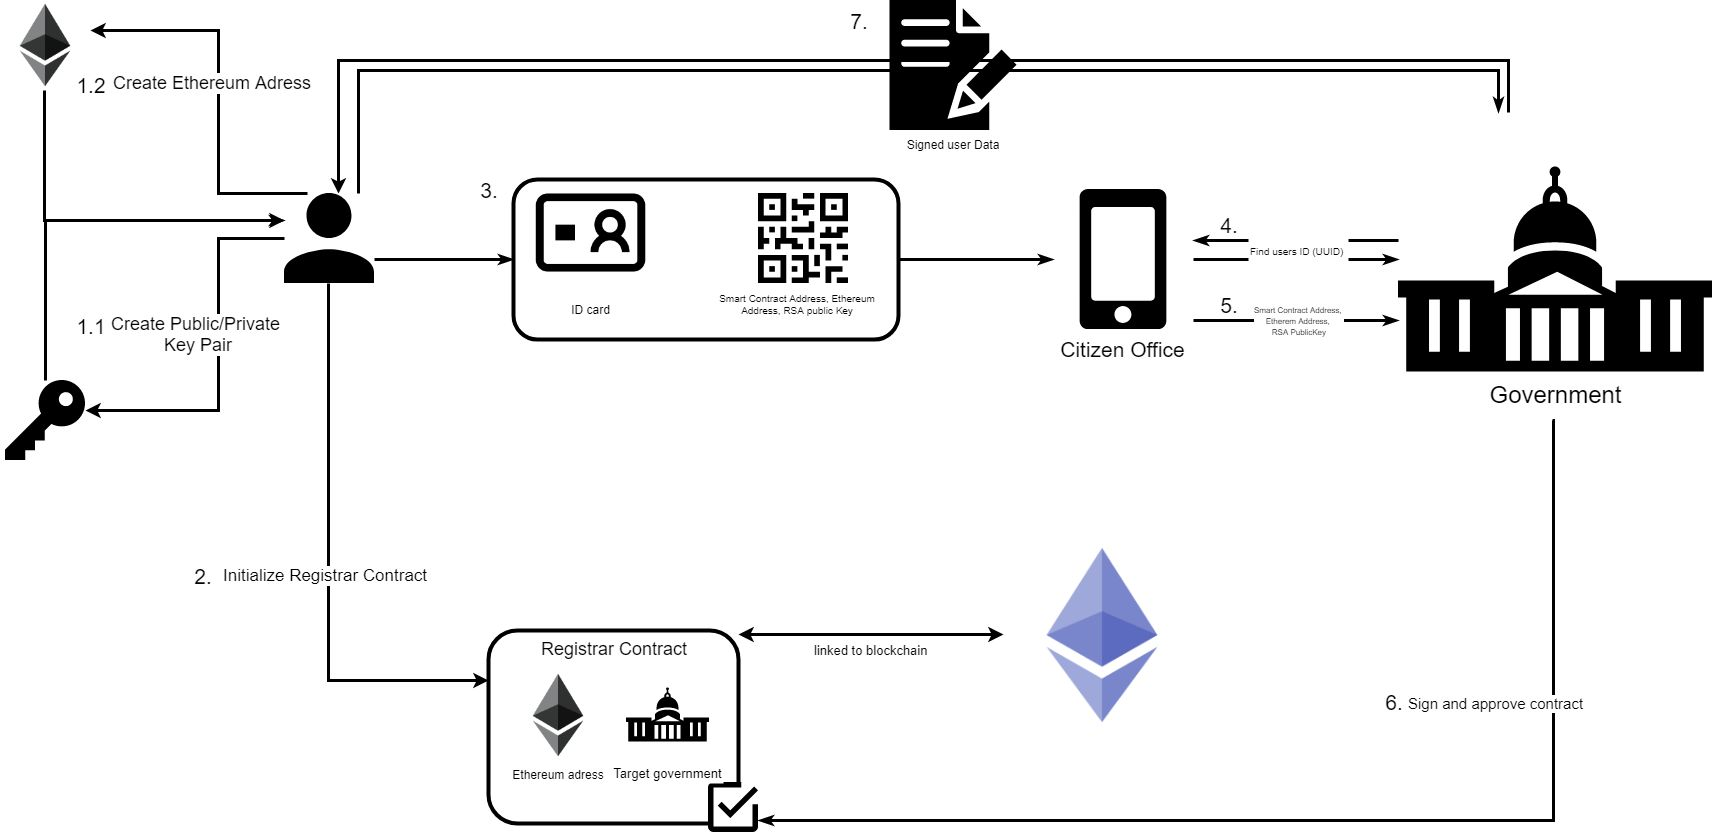
\includegraphics[width=\textwidth]{concept/registration_contract_general}
\caption{Registration}
\label{fig:registration_concept}
\end{figure}

\begin{enumerate}
\item \label{registrar_item_one}
The user creates an ethereum address and a private public key pair, the combination of these two are now used as the users digital identity. Jointly they act as a digital identity card. They are safely and securely stored in the users own database.
\item \label{registrar_item_two}
For verification and auditing purposes these have to be verified by a trusted party, so that third parties can be sure of the identity of the individuals.
We are using a specially designed smart contract, where the user inputs his ethereum address and his public key. Once filled, he writes it to the blockchain and waits for the trusted party, in our case a governmental agency, to check the contents, fulfill and sign the contract.
\item \label{registrar_item_three}
In order for that to happen, the user has to physically visit his citizen office with pre-existing identification documents. After verifying himself to the authorities they can use a specifically generated QR code to quickly check his digital identity.
\item \label{registrar_item_four}
With the information that is contained within the QR code the citizen office can now check their database for the corresponding entity.
\item \label{registrar_item_five}
After finding a corresponding user they extend their existing entity with the newly gathered ethereum address, the users RSA public key, and the registration contracts ethereum address.
\item \label{registrar_item_six}
The second to last step now is signing and approving the citizens registration contract.
\item \label{registrar_item_seven}
After approving the users registration contract the government creates a data blob containing all of the users information, signs it and lastly sends this signed user data to the user.
\end{enumerate}
The user is now a fully registered member within our community. Henceforth he can use this identity to request services and offer claims to and from other registered parties. 

\subsection{Permission Request}
With registration complete it is now time to use the system for its intended purpose. Meaning requesting services or purchasing goods from providers such as Banks, 
Car Rental Agencies, Airlines using \projectName{} for verification. In order to better understand how \projectName{} facilitates these transactions it is important to understand that
each identity is defined by an enormous amount of characteristics. These could be, but are not limited to, their given name, family name, age, full address, employer, e-mail address, physical characteristics such as facial structure, eye color, etc.
Each of these is mapped to a single so called claim within \projectName{}. In detail a claim represents a manifestation of one of these attributes. For example their given name could be Andrew or their eye color could be blue.
However just mapping these attributes to claims is not enough, they have to be verified by a trusted entity. To not set unrealistic expectations we focussed on information that has already been verified by the government in the form of an id card or other easily verifiable information such as
e-mail addresses. Lets continue on to the actual flow of how these claims are exchanged and afterwards there will be a brief explanation for why this flow was designed as shown. 

\begin{figure}[ht]
\centering
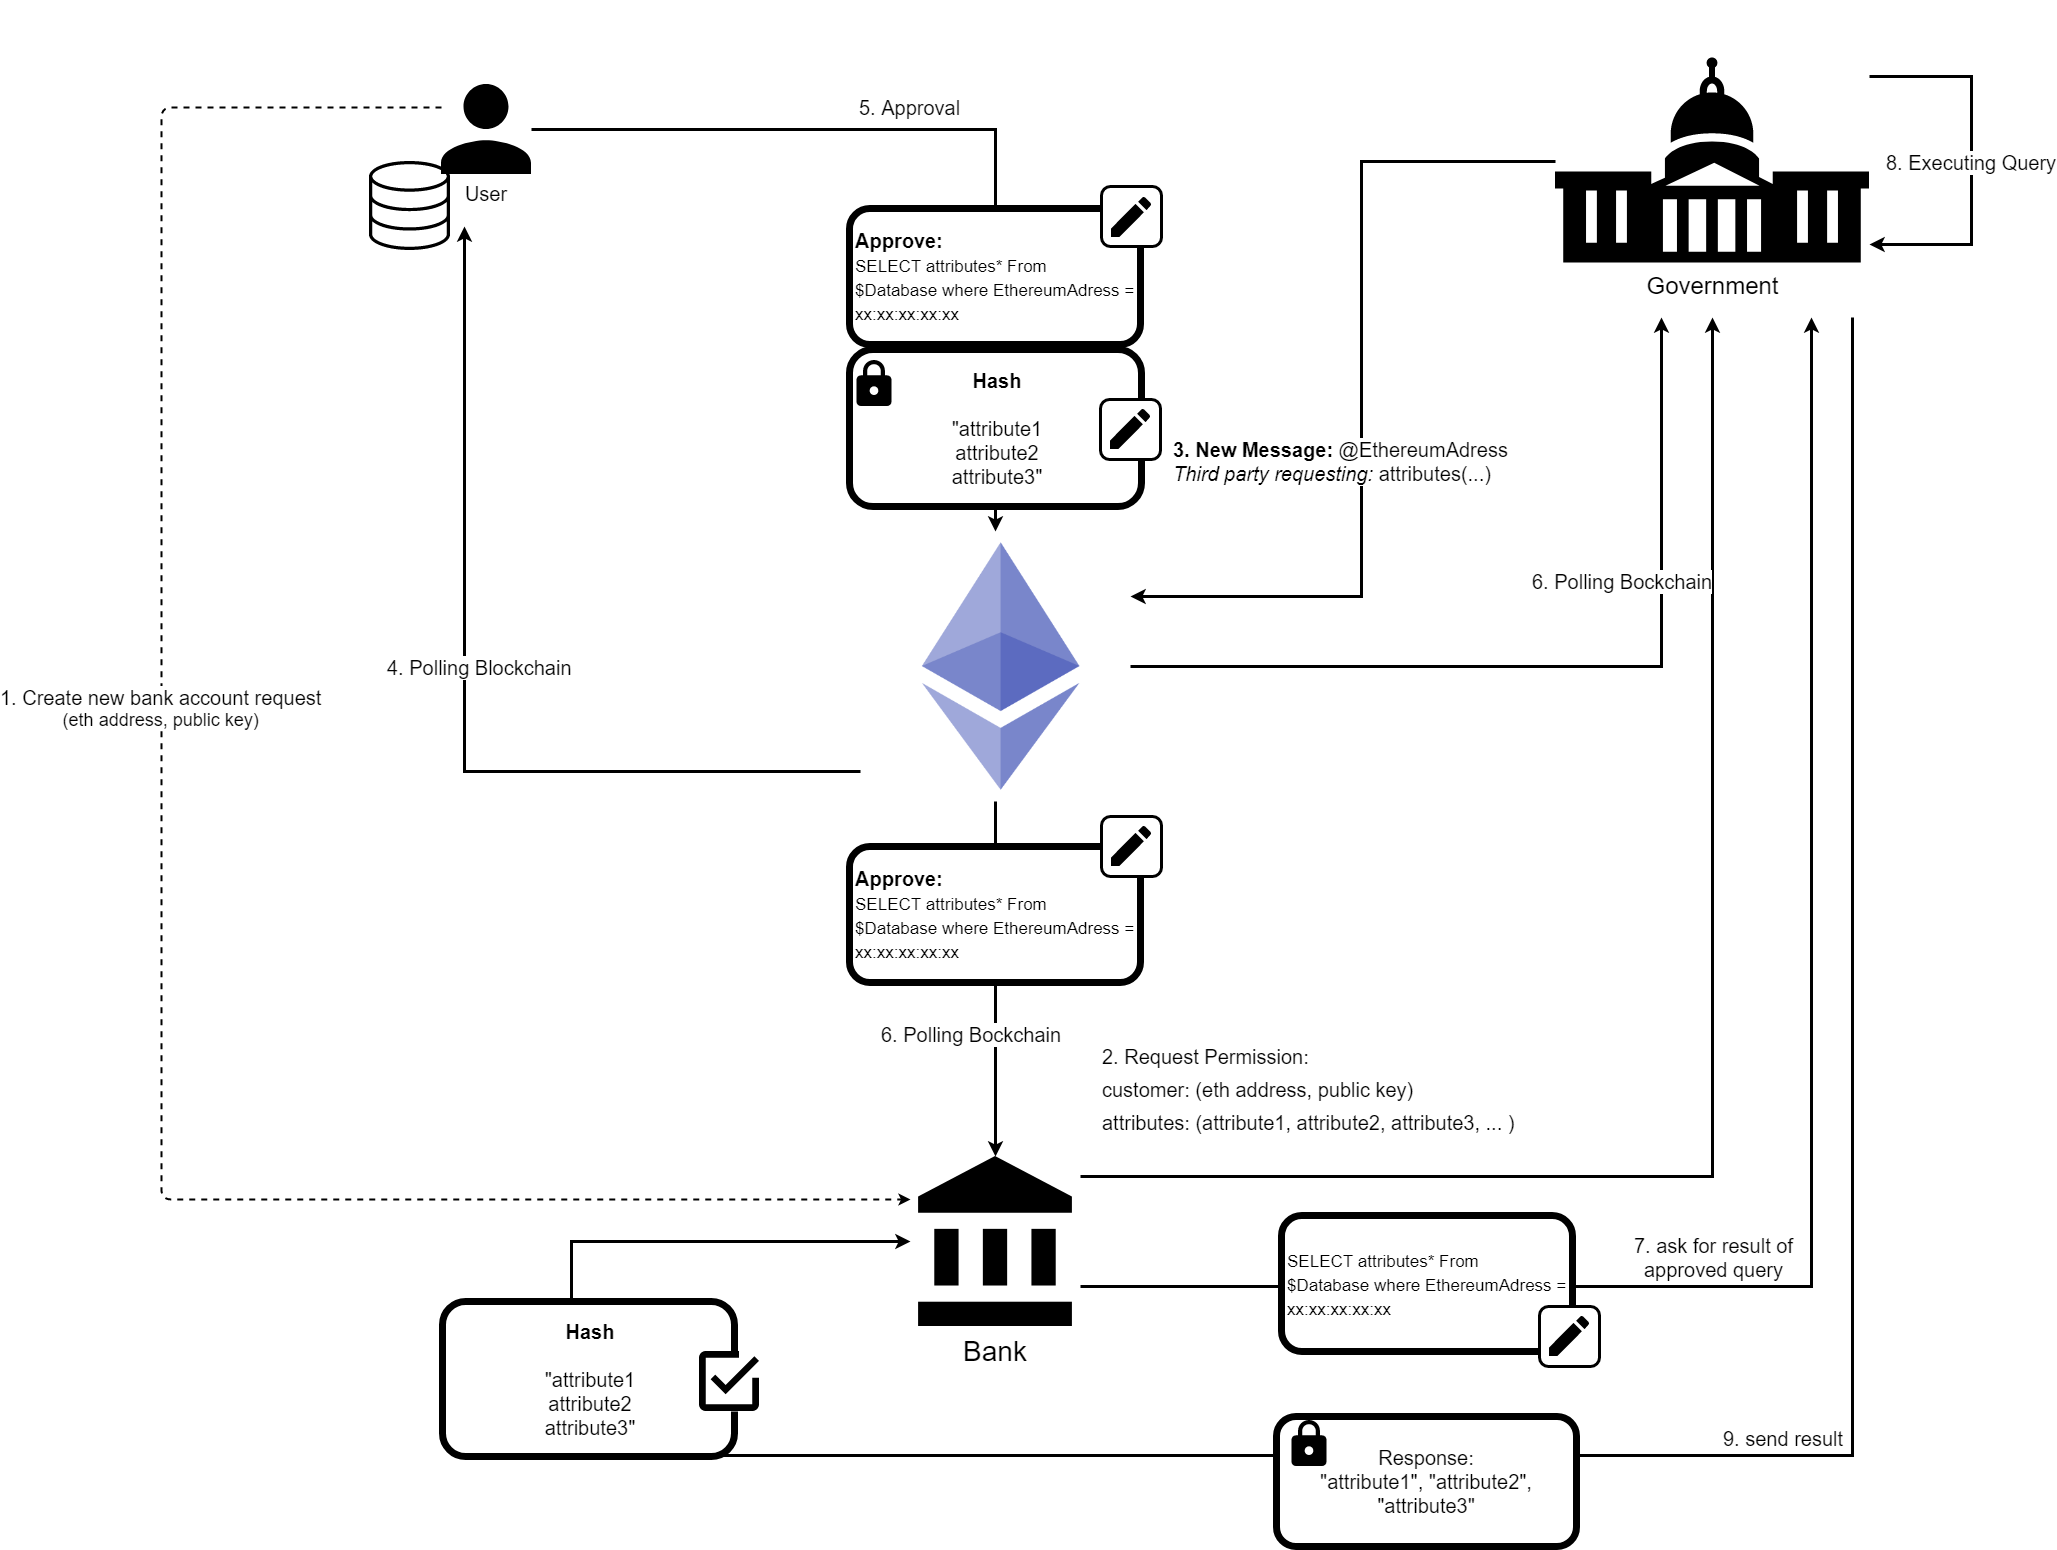
\includegraphics[width=\textwidth]{concept/permission_contract_general.png}
\caption{Permission Request}
\label{fig:permission_request}
\end{figure}

\begin{enumerate}
\item \label{permission_request_item_one}
The first step consists of a user requesting an actual service with his ethereum address and public key, in this example we are examining the creation of a new bank account.
\begin{comment}
"An" goes before all words that begin with vowels:
An egg
With two exceptions:
When "u" makes the same sound as the "y" in you, or "o" makes the same sound as "w" in won, then "a" is used:
a union
a united front
a unicorn
a used napkin
a U.S. ship
a one-legged man
https://english.stackexchange.com/questions/105116/is-it-a-user-or-an-user
\end{comment}
\item \label{permission_request_item_two}
The bank teller now enters that information into a \textbf{Request Permission} form additionally containing all claims that they deem necessary. These may contain claims such as
family name, given name, date of birth, current address, etc. After completion of the form it is sent to our trusted entity, the government, for further processing.
\item \label{permission_request_item_three}
The government now checks whether this user is part of \projectName{} and if successful creates a new message containing the target users ethereum address, requested claims and entity requesting the claims.
Therefore the message is loosely structured as follows:
\begin{itemize}
\item \textbf{EthereumAddress:} This is the users ethereum address
\item \textbf{ThirdPartyName:} The Banks name
\item \textbf{Requested claims:} Actually contains two separate arrays.
One holds all the required claims, without which the bank account registration will fail and the other contains optional claims.
These optional claims might be additional information that the bank would like to have for their data storage, but which also is not integral to creating a bank account.
\end{itemize}
\item \label{permission_request_item_four}
The user now polls the blockchain for new messages and finds this permission request by the bank.
\item \label{permission_request_item_five}
The user now checks each requested claim and decides whether he is willing to share these with the bank.
Since the claims importance, meaning whether they are required or optional, is visible, the user has full knowledge over his shared claims and information.
He may also decide that he isn't willing to share some required claims, knowing that his service request may be denied because of it.
\item \label{permission_request_item_five}
After this decision a signed query containing the shared claims and a signed hash of the shared claims is written to the blockchain.
\item \label{permission_request_item_six}
The government and bank notice the users answer and poll the blockchain for the new message.
\item \label{permission_request_seven}
The bank can now use the signed query to send it to the government for information retrieval.
\item \label{permission_request_eight}
The government checks the query against the blockchain and executes it.
\item \label{permission_request_nine}
After the query results are calculated the government sends a signed object containing the claims and their values, and a signed hash of these to the bank.
\end{enumerate}
After fully exploring how a permission request works in \projectName{} it is important to explain some of the pecularities of the design.
\begin{itemize}
\item \label{design_pecularity_one} \textbf{Why is it so convoluted?}
This is in part because it was our utmost priority to keep the users data as secure as possible while still allowing for information to be shared digitally.
This is however not just motivated by our own beliefs and opinions, but also because of the upcoming GDPR\ref{subsubsec:GDPR_compliance} regulation.
\item \label{design_pecularity_two} \textbf{Why use the blockchain at all if only a small amount of the user base is allowed to write to it?}
The main advantage of blockchain technologies are that they are based upon an open ledger concept. This basically means that every entity that is part of the network has full access to all entries in the blockchain.
This enables every entity to check for the flow of information and whether a transaction actually took place. Lastly all information that has been written is immutable which enables every participant to verify whether they are dealing with
fraudulent or correct information.
These concepts enable our system and allow us to stay within the tight regulations of the GDPR\ref{subsubsec:GDPR_compliance} while still offering identity services. Using the blockchain for transactional information instead of identity information
secures a users right to privacy while allowing him to share his information with third parties. Since third parties have read access, they can verify whether their requests have actually been sent to the user they are in contact with and
whether that user agreed to share his information with the third party.
In conclusion using the blockchains immutability and open ledger principles third parties can be sure that their requests have been handled and responded to, without the possibility of tampering after writing.
This enables every participant to acknowledge that some form of claim sharing has occured and is therefore verifiable.
Furthermore writing a permission request to the blockchain removes the possibility for third parties to alter their information requests after they have been sent and therefore increases the users trust in the system.
Mainly because users now have to give explicit consent to each and every single claim that is being requested without the possibility of third parties intervening and adding claims to the request after they have been granted or denied.
\item \label{design_pecularity_three} \textbf{Are there any additional benefits to handling information this way?}
The signed queries could be enriched with flags to increase functionality and usability. For example a user might define a query to only be usable x times or only to be valid up until a specific date in the future.
This further reinforces his right to self-sovereignity by only allowing access to his information for a limited time. 
\item \label{design_pecularity_four} \textbf{What are the costs associated with this process for the user?}
Users don't pay for the creation of the smart contract handling this information sharing request. However should claims change that have been shared as part of a permission request contract the user is financially responsible for the transaction costs of changing these signed claims.
\end{itemize}

% Please agument why the user if he is holding signed claims is not providing his claims directly to the requesting provider
% Include the following arguments:
% 1. request shell be populated through the blockchain so that every entity can acknowledge the claim sharing
% 2. populatring thre reuqest through the blockchain gives us the possibility to explicit approve the sharing
% 3. generating a signed query can also have additional attributes like a reuse flag to indicate if the query could be used again if the claim changed
% 4. user don't have to pay for the creation of the smart contract. only for the updating of the signed values



\subsection{Closures}
%Create closure figure in draw.io and insert here
\begin{comment}
\begin{figure}[ht]
\centering
\includegraphics[width=\textwidth]{concept/closure.png}
\caption{Closure}
\label{fig:closure}
\end{figure}
\end{comment}

\subsection{Changing Claims}

\begin{figure}
 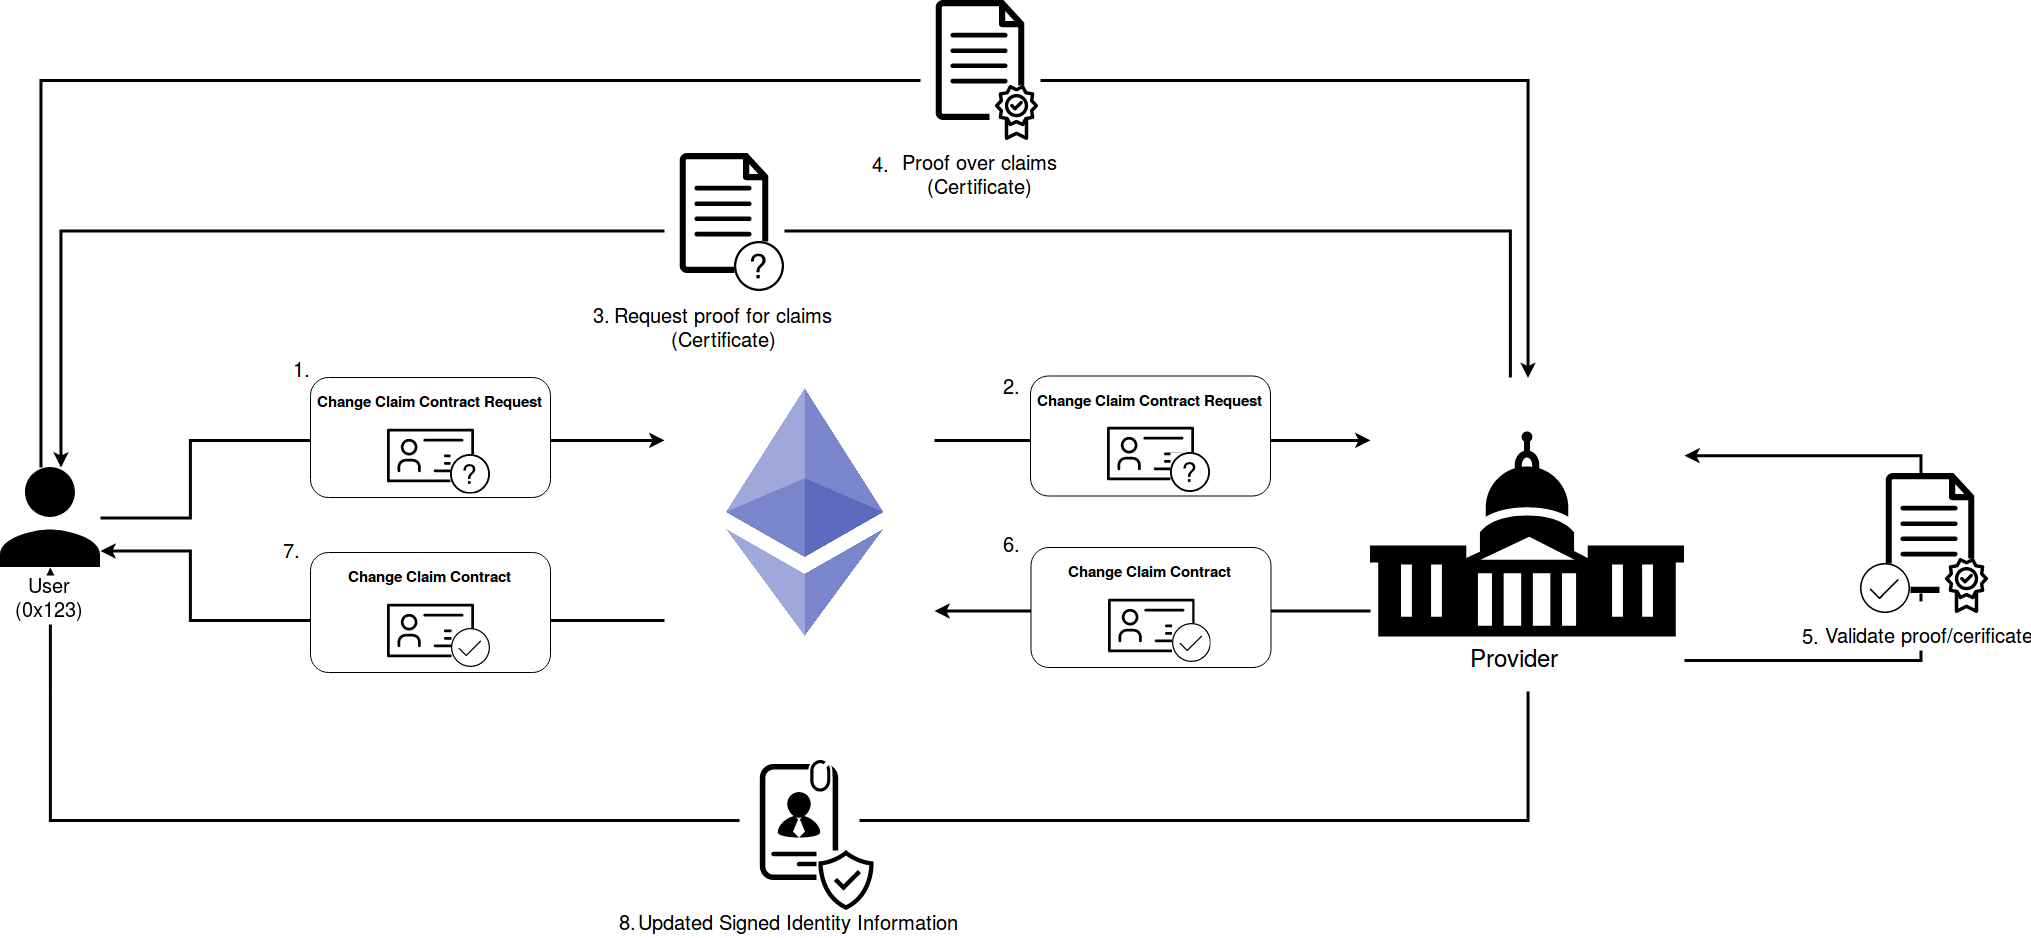
\includegraphics[width=\textwidth]{concept/change_claim.png}
 \centering
\caption{Concept of the change claim work flow. Change claim events are populated trough the blockchain so that every provider holding the same claim for the referenced user can start a new permission request to update the claim values.}
\label{fig:changeClaimsFig}
\end{figure}

Changing claims in a self-sovereign manner with still providing the high level of trust in this claims is a challenge. We evaluated two entry points for this contract: a) the user starts the procedure by sending a “change claim contract request” or b) the government enforces new claims by populating a “change claim contract”. 

Both actions are described as use cases in section \ref{sec:changeClaimUseCase}. For a) the use case that the user may want to change his family name because he got married recently. In the case of b) the government triggers a change claim as an law enforcement (e.g. the user looses his driving license for a certain time) or an other federal institution wants to update the users claims. Each scenarios are described in detail in this section. 

To still serve as a self-sovereign system the user gets the possibility to create a “change claim contract request” (step 1., figure \ref{fig:changeClaimsFig}). This contract itself does not enforce any change of any attributes, but serves as a change claim application. The user states the claim IDs he wants to change inside the contract. He may even add additional attributes like a time period to define for how long the claim shell be changed. It is also possible to propose new claims the user want to add by himself. However, new or changed claims needs to be verifiable by the provider. The “change claim contract request” is likely addressed at the institution that would have the highest trust level in the system, since the signature over this claims is only trusted as much as the institution itself. In our scenario the government satisfies this trust level. Some might argue that it is not necessary to populate the “change claim contract request” trough the blockchain (since each transaction cost money), but it helps to establish more transparency in our system and relocates power to the user. He decides which claims he wants to change and which new claims he wants to have added to his digital identity. 

The government pulls down the “change claim contract request” and evaluates, it in step 2., for which claims it needs a verification, e.g. a certificate. Off-blockchain the user is asked for a proof or certificate over his proposed claims (step 3.). Each provider can define which kind of proof the user must provide to get his claim changed. The level of trust in a provider grows with the amount of accuracy the provider puts in his claim validation. The user provides the proof in step 4. Since different provider may accept different proofs, it can be various documents, like photos of his ID card, certificates of his club membership or even audio recordings. However, if the user is not able to provide the necessary proofs, the contract will be killed and the change claim request rejected.
The provider validates if the provided proofs satisfies his acceptance criteria in step 5.  If the proofs are sufficient the provider accepts the “Change claim contract request” by setting a flag in the contract, or even removing some claims from the contract on which the verification failed (step 6.). 

Now every other provider in the system holding old claim values for the referenced user can create a new permission request to discover the new changed claims from the provider handling the change claim contract. The user still needs to approve the new incoming permission requests. In step 7. the user gets the notification about the successful approval of the change claim contract and queries the provider to retrieve a signed version of his updated claims (step 8.). 

Here the change claim process is finished. However, as mentioned previous there is also a scenario where a federal institution wants to enforce a claim change (for example the temporary removal of driving license). In that case we would directly start at step 6. where the government will publish an already approved “change claim contract” referring to the claim IDs that were changed and additional values restricting the duration of this enforcement. Extern observers of the blockchain will notice that it is an enforced claim change since the user did not provide a “change claim contract request”. In the same way as described previously, the provider will take note about the claim change and can setup a new permission request to discover the new claims. As a side note: If the user rejects the permission requests the providers holding outdated claim values can simply distrust this values and decide if they are still  willing to provide the user service with outdated values. Please referrer to section \ref{sec:changeClaimUseCase} for a use case.

\subsection{Evaluation}

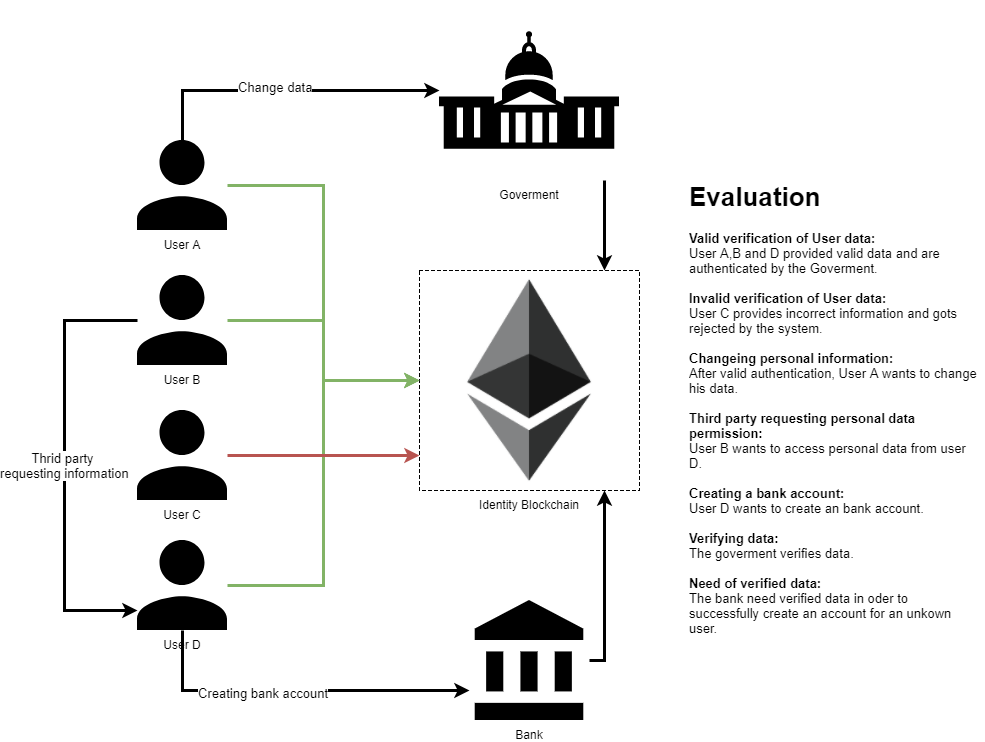
\includegraphics[width=\textwidth]{concept/evaluation.png}
 
\section{Use cases}

\subsection{Change a claim}
\label{sec:changeClaimUseCase}
\textbf{a) User changes claims:}
Lets have a user Bob Bobsen who has recently married Alice Alicson. Since Bob wants to change his family name to Bob Alicon this information needs to be updated in our system. To do so he creates a new “Change Claim Contract Request” holding the “FAMILY\_NAME” claim ID and addressing this contract to the government. The government will ask Bob for his marriage certificate. Bob sends his certificate over a secured connection to the government. They, on the other hand, can now verify the new claim by checking Bob's marriage contract. If the certificate is authentic the identity provider publishes an approve transaction to the change claim contract to notify all third parties and other identity providers about the new claim of Bob's digital identity.
Bob does then pull the blockchain, and requests the signed version of his new family name from the government, which he saves in his local database.

\textbf{b) Enforced claim changes:}
Bob has lost his driving license by a moderate traffic crime. Since Bob is still holding a signed version of his driving license in his local database he could easy rend a new car. So the government enforces a claim change by publishing a “Change Claim Contract” to the blockchain referencing Bobs ethereum ID, the driving license claim ID and a time period (6 month). Each entity observing the blockchain can within his 6 month distrust the driving license claim value provided by Bob, if the provided signature is older then the creation date of the “Change Claim Contract”. However, Bob can query the government for the updated claim value and retrieve the temporary restricted driving license, which is then also trusted, because it is up to date. After 6 month no new claim change contract needs to be setup because an entity can simply compute that the restriction time is expired and that no new claim change was published by the government. 
